\documentclass[draft]{agujournal2025}
\usepackage{booktabs}
\usepackage{amsmath}
\usepackage{tabularx}
\usepackage{ragged2e}
\usepackage{microtype}
\ifdefined\XeTeXversion\else
  \usepackage{seqsplit}
  \let\wrrtexttt\texttt
  \renewcommand{\texttt}[1]{\wrrtexttt{\seqsplit{#1}}}
\fi
\setlength{\emergencystretch}{3em}
%% Generated by scripts/367_wrr_revision_evidence.py
\newcommand{\RAdmissionCases}{70{,}011}
\newcommand{\RSourceNetworks}{193}
\newcommand{\RSourceGroups}{181}
\newcommand{\RSourceStations}{581}
\newcommand{\RSourceYears}{6{,}170}
\newcommand{\RSourceProviders}{10}
\newcommand{\RStratifiedCases}{40{,}232}
\newcommand{\REmpiricalCases}{29{,}779}
\newcommand{\RControlledCases}{406{,}015}
\newcommand{\RPriorControlledCases}{290{,}322}
\newcommand{\RPriorAdmissionCases}{46{,}510}
\newcommand{\RDocumentedControlledCases}{312{,}825}
\newcommand{\RDocumentedGroups}{144}
\newcommand{\RDocumentedYears}{4{,}720}
\newcommand{\RDeployableImprovement}{0.014}
\newcommand{\RDeployableLow}{0.008}
\newcommand{\RDeployableHigh}{0.019}
\newcommand{\RPosition}{0.62}
\newcommand{\RPositionLow}{0.58}
\newcommand{\RPositionHigh}{0.66}
\newcommand{\RLength}{0.13}
\newcommand{\RLengthLow}{0.10}
\newcommand{\RLengthHigh}{0.17}
\newcommand{\RInterpLength}{1.24}
\newcommand{\RInterpLengthLow}{1.12}
\newcommand{\RInterpLengthHigh}{1.35}
\newcommand{\RCompensatingSwitchShare}{60.4}
\newcommand{\ROracleRaw}{0.450}
\newcommand{\ROraclePermuted}{0.398}
\newcommand{\ROracleDemeaned}{0.215}
\newcommand{\ROracleBoth}{0.071}
\newcommand{\ROracleInteraction}{-0.091}
\newcommand{\RRetGainMin}{1.7}
\newcommand{\RRetGainMax}{3.8}
\newcommand{\RTargetDailyMin}{3.8}
\newcommand{\RTargetDailyMax}{6.2}
\newcommand{\RSmallSupportMin}{3.4}
\newcommand{\RSmallSupportMax}{9.5}
\newcommand{\RSplineSupportMin}{-1.2}
\newcommand{\RSplineSupportMax}{1.1}
\newcommand{\RPriorLocalGainMin}{4.1}
\newcommand{\RPriorLocalGainMax}{7.6}
\newcommand{\RWholeRetGain}{2.6}
\newcommand{\RWholeRetLow}{-1.9}
\newcommand{\RWholeRetHigh}{8.0}
\newcommand{\RWholeRetRefits}{1{,}000}
\newcommand{\RWholePriorGain}{2.9}
\newcommand{\RWholePriorLow}{-5.7}
\newcommand{\RWholePriorHigh}{11.3}
\newcommand{\RWholePriorRefits}{1{,}000}
\newcommand{\RNewDevelopment}{21}
\newcommand{\RNewCalibration}{13}
\newcommand{\RNewTest}{19}
\newcommand{\RNewStations}{53}
\newcommand{\RNewSwissTest}{7}
\newcommand{\RNewFrenchTest}{12}
\newcommand{\RTestRetFrozenRetention}{56.1}
\newcommand{\RTestRetFrozenRisk}{8.8}
\newcommand{\RTestRetRecalibratedRetention}{47.5}
\newcommand{\RTestRetRecalibratedRisk}{4.1}
\newcommand{\RTestRetLocalRetention}{44.4}
\newcommand{\RTestRetLocalRisk}{3.0}
\newcommand{\RTestRetCases}{669}
\newcommand{\RTestRetMagnitudeAbsoluteLoss}{0.1191}
\newcommand{\RTestRetMagnitudeVsAllUnknown}{0.0691}
\newcommand{\RTestRetMagnitudeLossDifference}{-0.3368}
\newcommand{\RTestRetMagnitudeLossLow}{-0.4059}
\newcommand{\RTestRetMagnitudeLossHigh}{-0.2720}
\newcommand{\RTestRetMagnitudeAbstentions}{294}
\newcommand{\RTestRetMagnitudeRescued}{0}
\newcommand{\RTestRetHotRefusal}{46.4}
\newcommand{\RTestRetCoolRefusal}{43.4}
\newcommand{\RTestRetOverallRefusal}{43.9}
\newcommand{\RTestRetJudgementAbsoluteLoss}{0.1190}
\newcommand{\RTestRetJudgementVsAllUnknown}{0.0690}
\newcommand{\RTestRetJudgementLossDifference}{-0.3369}
\newcommand{\RTestRetJudgementLossLow}{-0.4060}
\newcommand{\RTestRetJudgementLossHigh}{-0.2723}
\newcommand{\RTestRetJudgementAbstentions}{292}
\newcommand{\RTestRetJudgementRescued}{2}
\newcommand{\RTestRetTargetDailyGain}{9.4}
\newcommand{\RTestRetTargetDailyLow}{6.1}
\newcommand{\RTestRetTargetDailyHigh}{13.1}
\newcommand{\RTestPriorFrozenRetention}{47.4}
\newcommand{\RTestPriorFrozenRisk}{9.8}
\newcommand{\RTestPriorRecalibratedRetention}{37.0}
\newcommand{\RTestPriorRecalibratedRisk}{1.6}
\newcommand{\RTestPriorLocalRetention}{13.9}
\newcommand{\RTestPriorLocalRisk}{0.0}
\newcommand{\RTestPriorCases}{173}
\newcommand{\RTestPriorMagnitudeAbsoluteLoss}{0.0841}
\newcommand{\RTestPriorMagnitudeVsAllUnknown}{0.0341}
\newcommand{\RTestPriorMagnitudeLossDifference}{-0.4650}
\newcommand{\RTestPriorMagnitudeLossLow}{-0.6078}
\newcommand{\RTestPriorMagnitudeLossHigh}{-0.2935}
\newcommand{\RTestPriorMagnitudeAbstentions}{91}
\newcommand{\RTestPriorMagnitudeRescued}{0}
\newcommand{\RTestPriorHotRefusal}{48.8}
\newcommand{\RTestPriorCoolRefusal}{53.8}
\newcommand{\RTestPriorOverallRefusal}{52.6}
\newcommand{\RTestPriorJudgementAbsoluteLoss}{0.0838}
\newcommand{\RTestPriorJudgementVsAllUnknown}{0.0338}
\newcommand{\RTestPriorJudgementLossDifference}{-0.4653}
\newcommand{\RTestPriorJudgementLossLow}{-0.6081}
\newcommand{\RTestPriorJudgementLossHigh}{-0.2935}
\newcommand{\RTestPriorJudgementAbstentions}{90}
\newcommand{\RTestPriorJudgementRescued}{1}
\newcommand{\RTestPriorTargetDailyGain}{12.7}
\newcommand{\RTestPriorTargetDailyLow}{7.6}
\newcommand{\RTestPriorTargetDailyHigh}{17.1}
\newcommand{\RNaturalCases}{168}
\newcommand{\RNaturalGroups}{10}
\newcommand{\RNaturalPredictedRisk}{26.6}
\newcommand{\RNaturalObservedRisk}{21.4}
\newcommand{\RSingleThresholdGroups}{59}
\newcommand{\RGridThresholdGroups}{118}
\newcommand{\RBandSwissRet}{71.6}
\newcommand{\RBandSwissPrior}{60.7}
\newcommand{\RPhysicalThreeMAE}{0.254}
\newcommand{\RPhysicalThreeCases}{1{,}544}
\newcommand{\RPhysicalThreePolicyMAE}{0.280}
\newcommand{\RPhysicalEightMAE}{0.203}
\newcommand{\RPhysicalEightCases}{821}
\newcommand{\RPhysicalEightPolicyMAE}{0.342}

\newcommand{\tabletext}{\footnotesize\setlength{\baselineskip}{10pt}\setlength{\parindent}{0pt}}
\newcolumntype{Y}{>{\raggedright\arraybackslash}X}
\begin{document}
\journalname{Water Resources Research}
\title{When are incomplete river-temperature records fit for estimating thermal extremes?}
\authors{AUTHOR ONE\affil{1}}
\affiliation{1}{AFFILIATION PENDING AUTHOR CONFIRMATION}
\authoraddr{Corresponding author details pending author confirmation.}
\authorrunninghead{Ignored.}
\titlerunninghead{Ignored.}
\keypoints
  {Equal gaps have different peak-temperature consequences, but length still matters and window switching can compensate cold errors}
  {Extra peak-window features do not show a stable practical gain beyond direct uncertainty in the hottest 30-day mean}
  {Frozen transfer does not validate its risk target; local calibration, unknown records and refusal costs change a screen's value}
\maketitle

\begin{abstract}
An incomplete river-temperature record can be adequate for one use and inadequate for another. We evaluate this distinction for the annual hottest consecutive 30-day mean, H30, using \RSourceYears{} complete reference station-years and separate mechanism, admission and recorded-calendar experiments. Equal 30-day gaps overlapping the climatological peak increase climatology-based H30 absolute error by \RPosition{}\,$^{\circ}$C relative to gaps outside it, but length retains an effect, especially for interpolation. An exact decomposition separates true-window error from a nonnegative window-switch increment; switching often compensates underestimation rather than creating an excessively hot peak. A proposed uncertain-window score combines conditional peak support, competing windows and reconstruction reliability. Its source-admission gain over a matched generic score is \RRetGainMin{}--\RRetGainMax{} percentage points, below the predefined five-point practical margin, and direct H30 uncertainty accounts for essentially the same gain. Models and thresholds are frozen before testing new station histories. On \RTestRetCases{} Swiss documented-mean cases, the score retains \RTestRetFrozenRetention{}\% but incurs \RTestRetFrozenRisk{}\% failures, exceeding its 5\% calibration target; local recalibration lowers point risk to \RTestRetRecalibratedRisk{}\%. Screening can reduce locally anomalous-hot classification loss under declared refusal costs, without establishing universal management benefit. Target-specific diagnostics, additional window representation, transferable risk control and downstream value require separate evidence.
Always-unknown answers can be cheaper than the screen under this loss.
\begin{plainlanguagesummary}
Missing temperature observations do not all have the same consequences. A gap during a river's hottest weeks can change its estimated hottest month much more than an equally long gap elsewhere. That does not make the number of missing days irrelevant. We test both effects and compare rules that decide whether to report a reconstructed peak. A more elaborate representation of the uncertain peak window does not reliably improve on uncertainty in the peak temperature itself. A rule calibrated on existing records also makes too many errors when transferred unchanged to new Swiss records. Calibrating with local examples helps, but the number of independent rivers is too small to guarantee a low error rate. Refusing a numerical estimate is not the same as declaring a cool year. Its practical value depends on what managers need to know and how costly an unknown answer is.
\end{plainlanguagesummary}
\end{abstract}
\section{Introduction}
River-temperature records support habitat assessment, thermal classification and description of climatic extremes \cite{caissie2006}. These uses do not ask for the same property of the daily series. The hottest consecutive 30-day mean, H30, can be sensitive to an outage near a thermal peak despite high annual coverage. Conversely, a substantial outage may leave enough information for a particular hot-year judgement. The question is whether remaining information supports the intended decision.

This question has an important literature. \citeA{johnson2021} examined missing-data timing and annual stream-temperature analyses; \citeA{beaufort2022} reconstructed thermal peaks from heterogeneous records and explicitly used seasonal information. Neither the importance of season nor evaluation of a derived thermal statistic originates here. Selective prediction already exchanges prediction coverage for user-specified error risk \cite{geifman2017}, and learning a score before testing acceptance rules is established practice \cite{angelopoulos2025}. The application problem is whether a target-window representation adds information beyond strong reconstruction diagnostics, and whether a source-trained admission policy remains reliable and useful elsewhere.

The true peak window is hidden, whereas a historical climatological window is available to an agency. Removing explicit overlap does not remove every implicit source of peak information: calendar position, coverage and reconstructed-H30 disagreement can encode it. Low pooled error can coexist with failures in particular rivers. A precise H30 number and a correct hot-year label are also different outputs. Improvement in one cannot be assumed to improve the other.

We link five evidence groups: paired recovery, an error identity and residual interventions, same-information comparisons, frozen new-station transfer, and original-candidate decisions. Hypotheses and falsifiers were written before new experiments (Table~\ref{tab:hypotheses}). Opened sources remain development evidence, however broad their coverage. Negative findings are permitted rather than replaced by a favorable endpoint.

\begin{table}
\caption{Questions fixed before new experiments. Failure means absolute H30 error above 0.5\,$^{\circ}$C. The empirical calibration target is 5\%, not a guarantee of deployment risk.}
\label{tab:hypotheses}
\centering
\tabletext
\begin{tabularx}{\textwidth}{p{0.06\textwidth}YYY}
\toprule
 & Hypothesis & Required comparison & Falsifier \\
\midrule
H1 & Target-window information helps beyond missing-day and flexible seasonal summaries & Paired timing/length controls; matched small and flexible models & No reproducible increment over seasonal comparators; an explicit-feature ablation alone is insufficient \\
H2 & Uncertain support, reliability and competition give a practical admission gain & Same learner, point, labels and calibration; generic H30, direct uncertainty and certificate references & No independent gain beyond five retention points at the common risk target; equivalence uses a separate two-point margin \\
H3 & Admission improves a locally hot-year decision & Identical original pool; reconstruction, screening, classification and charged abstention & No improvement over reconstructing all under declared positive abstention costs; lost information cannot be hidden \\
\bottomrule
\end{tabularx}
\end{table}
\section{Reference records and experiments}

\subsection{Opened sources and a new-station test}

The opened-source cohort comprises \RSourceStations{} provider-station identities, \RSourceYears{} distinct complete station-years and \RSourceNetworks{} network labels from \RSourceProviders{} providers. Shared target or donor records connect labels into \RSourceGroups{} record-overlap components: labels are not independent replications. The primary measurement scope requires provider-documented daily means; uncertain daily statistics and project aggregation are sensitivities. The documented-mean controlled experiment contains \RDocumentedControlledCases{} masks on \RDocumentedYears{} station-years in \RDocumentedGroups{} components. Completeness means every calendar-day reference value is finite, not that sensors are physically error-free or providers never estimated daily values.

For new histories, we began with the mountain-river resource accompanying \citeA{vanhamel2024,vanhameldata2024}. Its extreme-value subset is not a continuous H30 reference. We reacquired continuous temperatures from Swiss FOEN and French Hub'Eau. All previously used target \emph{and donor} identities were audited, including aliases, coordinates and available catchment connections. Candidate components received salted development, calibration and test roles before daily values were acquired. Completeness and the full prior-input audit subsequently reduced eligibility, without reshuffling roles or selecting on performance.

The cohort contains \RNewStations{} stations: \RNewDevelopment{} development, \RNewCalibration{} calibration and \RNewTest{} test. The latter include \RNewSwissTest{} Swiss documented-mean and \RNewFrenchTest{} French project-aggregated records. French daily values require at least four observations spanning eighteen hours in local time; source qualification includes explicitly unqualified observations, so they do not replace the primary measurement scope. Four complete reference years are required, with at least three permitted complete training years for an evaluated year. Acquisition and exclusions are in supporting information (SI).

These are new histories, not necessarily new institutions. European source and target records are station-disjoint after audit, but old catchment polygons are incomplete. USGS-only source models provide a further frozen transfer without shared source-target river-flow connections. They do not remove climatic dependence or shift. Glacier and snow attributes support descriptive strata, not verified groundwater or regulation classes. Snow share is a percent: the corrected majority-snow threshold is 50\%, assigning glacier influence first. That descriptive correction changes no predictor, threshold, record or frozen role.

\subsection{Mechanism and admission are different populations}

For mechanisms, 30-, 60- and 90-day gaps have feasible zero, partial or full overlap with the training-only climatological peak window. Four start realizations are attempted per station-year cell. Warm-season controls hold missing warm-season days fixed; fragmented and contiguous masks have equal total warm missing-day budgets. Infeasible cells remain empty. All measurement classes yield \RControlledCases{} retrospective and \RPriorControlledCases{} earlier-years-only cases. More masks improve placement resolution, not independent river replication.

This long-gap population is unsuitable as primary admission evidence: omitting short outages can make a length rule reject everything. Admission instead regenerates target lengths 14, 30, 60, 90, 120, 180 and 270 days, one feasible climatological-overlap class per length, and up to five transplanted empirical geometries. The retrospective cohort contains \RAdmissionCases{} cases, comprising \RStratifiedCases{} single-run and \REmpiricalCases{} empirical geometries; earlier-years-only reconstruction gives \RPriorAdmissionCases{}. This is a constructed assay, not natural outage prevalence. Earlier controlled-panel classifier fits remain diagnostics, not the admission headline.

Recorded-calendar replay transfers genuinely incomplete historical shapes onto complete reference years. It does not observe the original incomplete years' unknown values and excludes calendars with no missing or no observed days. Equal-duration event masks fall before, during and after the same longest thermal episode. Project episodes exceed a training-only seasonal 95th percentile for at least three days; published events use a separate two-day definition. Compound heat/low-flow labels use training-month discharge quantiles. Discharge missing on required gap-event days remains unknown.

We cross timing with removal of none, half or all initially usable neighbours, recomputing local reconstruction inputs but leaving admission heads and thresholds unchanged. Fractional removal rounds upward, so a one-neighbour case loses it at both nonzero levels. The new European bundles are single-station: their cofailure contrast would be degenerate. The nondegenerate test uses held-out opened-source multi-station components. Event-dependent masking is informative-missingness stress, not identification of real instrument-failure causes.

\section{Decision-time methods and validation}

\subsection{Estimand, reconstruction and error channels}

For a complete recorded year $y$,
\begin{equation}
H_{30}(y)=\max_{w\in\mathcal W_{30}}\frac{1}{30}\sum_{t\in w}y_t,
\end{equation}
where $\mathcal W_{30}$ contains consecutive windows within that calendar year. Let $M$ denote missing days and $S$ a maximizing true window. A climatological window $S_c$ uses only permitted history. Its overlap $|M\cap S_c|/30$ is available at decision time; true overlap $|M\cap S|/30$ is an evaluation diagnostic, never a screening feature.

We fit day-of-year and smooth climatologies, interpolation, neighbour ridge and air-temperature ridge. The common point follows a fixed information priority: usable neighbour prediction, available air prediction, interpolation if the actual longest run is at most 30 days, then smooth and day-of-year climatology. Every hidden day must receive a finite value; observations stay unchanged. This is an information-priority policy, not selection on hidden error. Individual reconstructors and a certificate choosing its own method are separate comparisons.

Writing $\widetilde y$ for a completed year and $\widehat S$ for its maximizing window gives
\begin{align}
H_{30}(\widetilde y)-H_{30}(y)&=B+F,\\
B&=\frac{1}{30}\sum_{t\in S}(\widetilde y_t-y_t),\\
F&=\overline{\widetilde y}_{\widehat S}-\overline{\widetilde y}_{S}\geq0.
\end{align}
$B$ is error carried by the true window, with zero contribution from observed days. $F$ is a \emph{window-switch increment}. Another observed window can replace an underestimated true peak, making $F$ positive while final error stays negative. It is not generally a false-hot-peak channel. A stratified absolute-error association between aligned and misaligned windows is not identified with $F$.

We cross hidden-residual permutation with removal of their hidden mean, including the interaction. Both require truth. A separate deployable correction uses visible flanks and historical residual information with shrinkage. Oracle centering benefits are not operational improvements or evidence of unconditional physical cold bias: conditioning on a true maximum can favor negative error there.

\subsection{Conditional trajectories and matched comparators}

Leave-training-year-out prediction residuals supply contiguous blocks for 128 conditional completed trajectories around the policy reconstruction. Blocks are nominally fourteen days and never bridge missing residual runs. If none exists for a shorter interpolation gap, a complete block as long as its longest run is permitted; long gaps never fall back to independent singletons. Observations stay fixed. Trajectories yield H30 spread/error-scale summaries, probabilistic hidden support, peak-location dispersion, competition and interactions. Bands are raw scenarios, not confidence or risk guarantees.

The uncertain-window score adds window summaries to a generic model containing gap, season, history, donor and reconstructed-H30 disagreement features, plus direct H30 uncertainty. Primary comparisons share quantile boosting, capacity, labels, point and calibration resources. Alternatives include direct H30 uncertainty; actual out-of-fold daily reconstruction scale; complete historical/observed diagnostics; mask-matched historical H30 error; seasonal splines; and small logistic models with and without overlap. Replacing H30 disagreement with daily prediction disagreement tests target awareness, not just explicit overlap. Removing competition, window spread and donor features tests the components.

A common-point certificate proxy differs from an aligned head for the current policy. A whole-system certificate chooses its own reconstruction and calibrates that point's error; it is not a feature-only comparison. Unsupported scores do not remove candidates. Air2stream-3/8 \cite{piccolroaz2016} and an old-source-trained univariate CSDI reference \cite{tashiro2021} test reconstruction sensitivity on identical masks, with availability and matched-subset policy errors. CSDI has no fully prospective claim. Air2stream forcing calibration and normalization exclude the target year and use earlier years prospectively. Extra meteorology, discharge or neighbours are information increments, not architectural gains.

\subsection{Calibration, transfer and the independent unit}

Source comparisons use five outer folds with disjoint fitting, calibration and testing components in approximately 60/20/20 proportions, repeated for three seeds. Candidate thresholds are fixed from training scores. The empirical selector uses a calibration component bootstrap and is heuristic. A zero-failure bootstrap can return zero uncertainty without assigning probability to an unseen failure type; more repetitions do not solve that problem.

For a formal alternative, let $A_g$ be within-component mean admission and $B_g$ mean admission times failure. Test $X_g=B_g+0.05(1-A_g)$. A Chernoff--KL upper bound on $E[X_g]$ at most 0.05 implies $E[B_g]/E[A_g]\leq0.05$, with positive denominator. Bonferroni adjustment permits searching training-fixed candidates without monotonic-risk assumptions. This requires independent, deployment-representative components and a predictor independent of calibration. It concerns a group-expectation ratio, not every subgroup, arbitrary archive case risk or unconditional transfer. Even with zero failures and full admission, one threshold needs \RSingleThresholdGroups{} independent groups; 21 candidates need \RGridThresholdGroups{}. Our target calibration cohorts cannot establish this guarantee.

Deployment separates F0, unchanged source model and threshold; F1, the same model with target calibration; and F2, new-development fitting with target calibration. Provider-excluded and USGS-only transfers are further checks. Local historical reconstruction fitting is allowed; hidden target-year labels never select a method. Predictive choices are hashed before target calibration errors; thresholds are locked before test errors.

Earlier-years-only local reconstruction is not a complete forward-in-calendar-time pipeline. Our forward experiment also fits and calibrates the global head through 2018, evaluates 2019--2022, and computes local climatology, donor relationships and residual diagnostics from earlier calendar years. This is a retrospective forward hindcast using current-vintage observations and reanalysis, not a real-time-vintage or prospective field trial; historical publication and revision vintages are unavailable. Its smaller pool is separate. Whole-procedure uncertainty refits learning and calibration in \RWholeRetRefits{} component resamples per protocol, unlike intervals conditional on fitted procedures. Learning curves use repeated subsets. Power projections retain training/calibration variability and do not establish common-risk feasibility under shift.

\subsection{Downstream loss and refused records}

The primary label asks whether H30 exceeds the 90th percentile of permitted training-year H30. This finite-history local anomaly proxy is not a verified ecological or regulatory standard. Fixed 18 and 20\,$^{\circ}$C labels are sensitivities. False-hot, missed-hot, correct and unknown outcomes share the original pool, with separate hot/cool refusal, threshold proximity, coverage and regional-frequency distortion.

With false-hot cost one, loss is $(c_{FN}FN+FP+c_AU)/N$. Declared missed-hot costs are 1, 5 and 10; unknown-answer costs are 0, 0.01, 0.025, 0.05, 0.1 and 0.25. Refused records remain unknown or interval-valued, not automatically repaired. These are not measured agency preferences; intervals across the grid are descriptive, not simultaneous guarantees.

A refused magnitude can retain an identified hot label. Let $L$ be the largest mean of a \emph{fully observed} 30-day window, or minus infinity if none exists. Since $L\leq H_{30}(y)$, $L$ above threshold establishes hot conditions against the complete recorded reference. An 80\%-observed mean is not a bound. This secondary rescue leaves magnitude admission unchanged. Observation margins of 0.1 and 0.2\,$^{\circ}$C are scenarios, not certified sensor bounds; $L$ below threshold never establishes cool conditions.


\section{Results}

\subsection{Position matters, without making length irrelevant}

In documented means, moving a 30-day gap from zero to full climatological overlap raises climatology H30 absolute error by \RPosition{}\,$^{\circ}$C [\RPositionLow{}, \RPositionHigh{}] (Figure~\ref{fig:recovery}). The broadened and warm-season controls show that this is not confined to the earlier small provider subset. Its magnitude nevertheless depends on reconstruction and auxiliary information (SI Tables S4--S6).

Length retains an effect. Where the true peak is entirely hidden, extending 30 to 90 days raises climatology error by \RLength{}\,$^{\circ}$C [\RLengthLow{}, \RLengthHigh{}], and interpolation error by \RInterpLength{}\,$^{\circ}$C [\RInterpLengthLow{}, \RInterpLengthHigh{}]. Fragmentation changes true support exposure despite equal total warm missing days. These contrasts do not support an assertion that only peak-window hiding damages H30, or that length and method rankings are invariant. Target-aware assessment is warranted; one overlap number is not a sufficient replacement for completeness information.

\begin{figure}
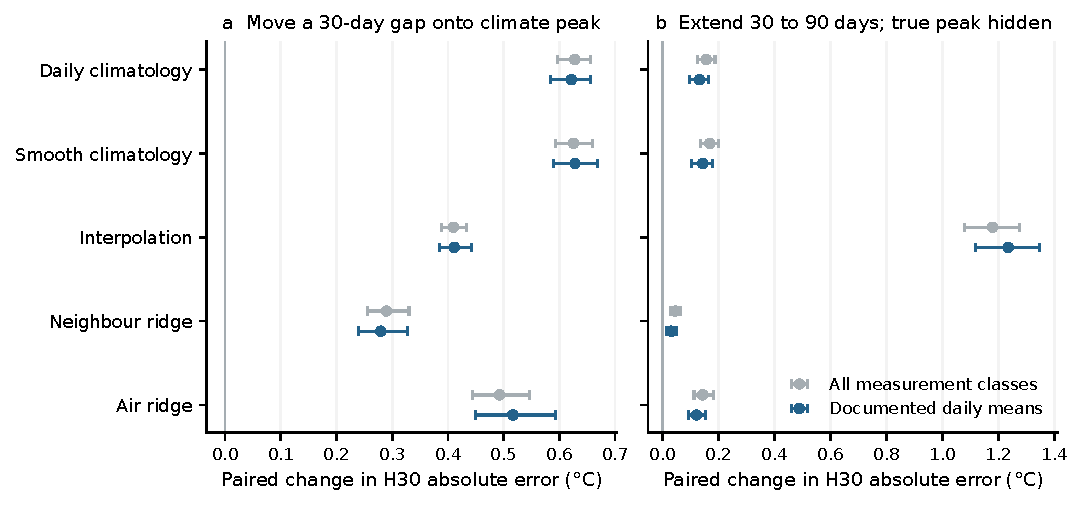
\includegraphics[width=\textwidth]{figures/r3_f1_recovery.pdf}
\caption{Paired mechanism contrasts. (a) Full-minus-zero climatological overlap for equal 30-day gaps. (b) Extension from 30 to 90 days with the true peak entirely hidden. Blue denotes documented daily means, gray all measurement classes; bars are component-bootstrap intervals. Starts are averaged within station-years, not counted as independent rivers.}
\label{fig:recovery}
\end{figure}

\subsection{An identity does not itself identify a deployable remedy}

The identity holds to numerical precision and the switch increment is nonnegative (SI Table S7). Among positive climatology increments, \RCompensatingSwitchShare{}\% still end below true H30. Switching often buffers cold errors rather than fabricating hot extremes (Figure~\ref{fig:channels}).

Climatology oracle mean absolute errors are \ROracleRaw{}\,$^{\circ}$C originally, \ROraclePermuted{} after permutation, \ROracleDemeaned{} after centering and \ROracleBoth{} after both. The interaction is \ROracleInteraction{}\,$^{\circ}$C, so improvement percentages are not additive mechanism shares. The visible-information correction improves policy MAE by only \RDeployableImprovement{}\,$^{\circ}$C [\RDeployableLow{}, \RDeployableHigh{}]. The oracle diagnoses structure without demonstrating a large available correction.

\begin{figure}
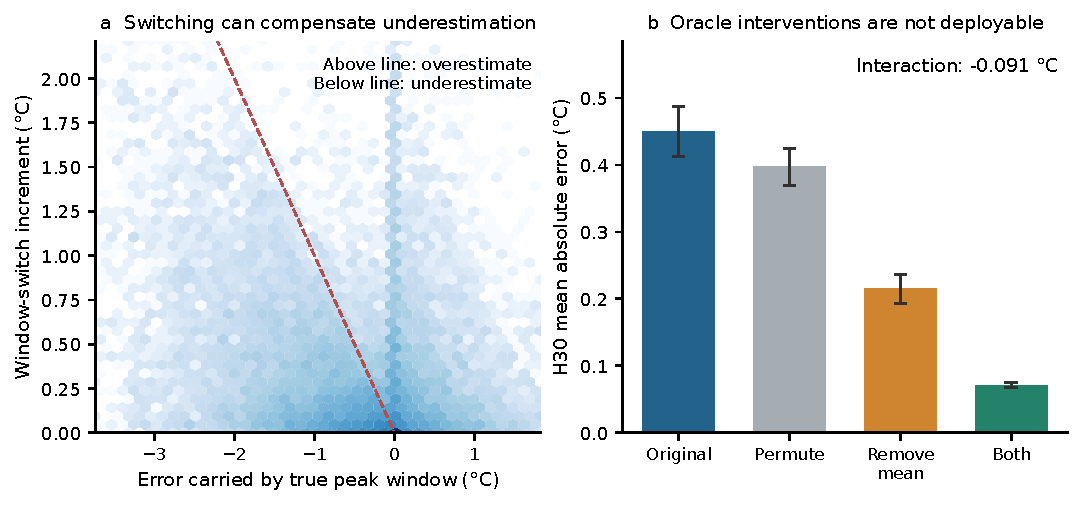
\includegraphics[width=\textwidth]{figures/r3_f2_channels.pdf}
\caption{Error structure and operational limits. (a) Climatology true-window error versus switch increment in documented-mean, replicate-zero controlled masks. The diagonal separates net under- and overestimation; axes show the central 99\% range. (b) Truth-dependent factorial interventions with component-bootstrap intervals. Their interaction is nonzero. The small deployable improvement is reported separately, not inferred from these bars.}
\label{fig:channels}
\end{figure}

\subsection{Direct target uncertainty explains the representation's gain}

On the admission mixture, uncertain-window source retention improves over the matched H30-generic score by \RRetGainMin{}--\RRetGainMax{} points across seeds, not the predefined five-point practical gain (Figure~\ref{fig:information}). Earlier-years-only \emph{local-input} comparisons give \RPriorLocalGainMin{}--\RPriorLocalGainMax{} points, but are not a global forward pipeline. In the fully refitted calendar-time forward experiment, the mean difference is \RWholePriorGain{} points with whole-procedure interval [\RWholePriorLow{}, \RWholePriorHigh{}]. Retrospective whole-procedure uncertainty is also broad: \RWholeRetGain{} [\RWholeRetLow{}, \RWholeRetHigh{}].

Direct H30 uncertainty gives essentially the same conditional source retention as the larger window representation. Their conditional paired intervals lie within the predefined two-point equivalence band, whereas whole-procedure intervals do not establish equivalence. Complete historical diagnostics are also competitive. This distinguishes target-specific diagnostics from a necessary uncertain-window representation, not models with and without all peak information. Small-model support features, flexible seasonal alternatives, daily-versus-H30 disagreement and component removals appear together (SI Tables S9--S13), rather than selecting a favorable ablation.

Target awareness nevertheless has identifiable value. Replacing daily disagreement with H30 disagreement improves source retention by \RTargetDailyMin{}--\RTargetDailyMax{} points with matched learner and reconstruction information. On independent Swiss records after local recalibration, the difference is \RTestRetTargetDailyGain{} points [\RTestRetTargetDailyLow{}, \RTestRetTargetDailyHigh{}]. Explicit overlap adds \RSmallSupportMin{}--\RSmallSupportMax{} points to the small logistic model, but its increment to the seasonal spline ranges from \RSplineSupportMin{} to \RSplineSupportMax{} points. H1 therefore supports target-specific diagnosis, not a universally necessary overlap variable or a demonstrated small-data advantage over flexible seasonal representations.

The trajectory scores are not calibrated probabilities. Raw 90\% scenario-band coverage is only \RBandSwissRet{}\% in retrospective Swiss admission and \RBandSwissPrior{}\% prospectively. Their representation comparison does not establish that a better joint predictive distribution could never make window information useful.

\begin{figure}
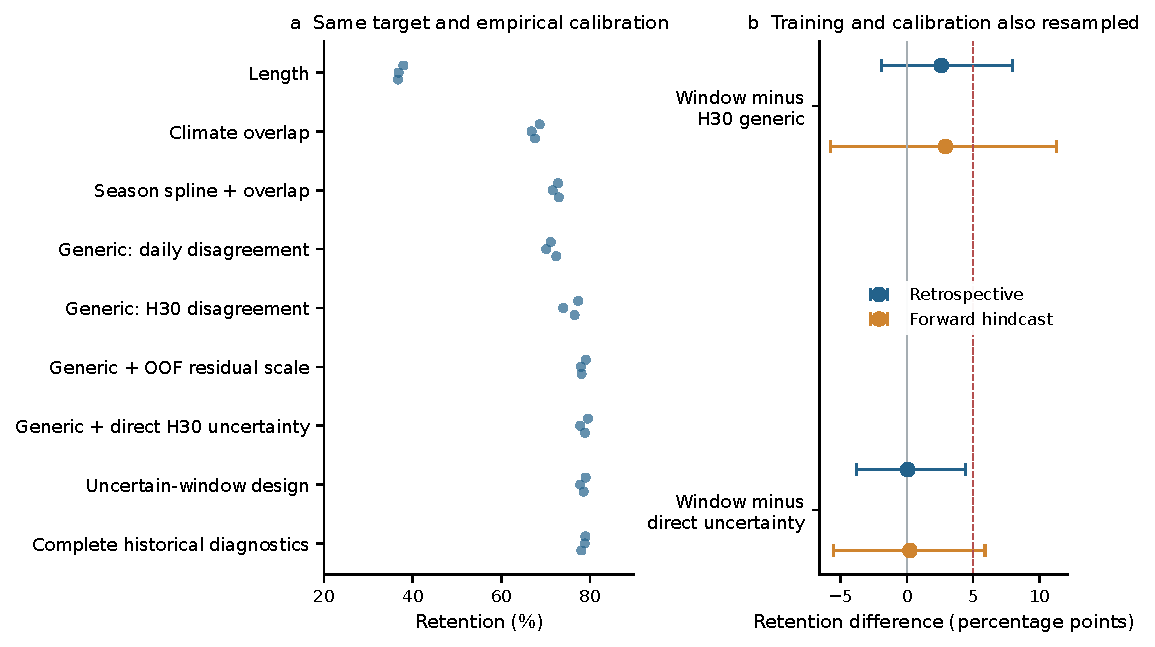
\includegraphics[width=\textwidth]{figures/r3_f3_information.pdf}
\caption{Contribution attribution on the admission cohort. (a) Retention under the common empirical calibration target; each dot is a split sensitivity, not independent replication. OOF denotes out-of-fold residuals of the actual reconstructor. (b) Whole-procedure intervals refit learning and calibration and resample evaluation components. The dashed line is the five-point superiority margin. Small conditional differences do not imply whole-procedure equivalence.}
\label{fig:information}
\end{figure}

\subsection{Independent transfer does not establish its calibration target}

On \RTestRetCases{} Swiss documented-mean cases from \RNewSwissTest{} held-out components, uncertain-window F0 retains \RTestRetFrozenRetention{}\% with \RTestRetFrozenRisk{}\% failures (Figure~\ref{fig:transfer}). Unchanged transfer therefore misses the nominal 5\% target at its observed operating point. Seven-component intervals do not establish that population risk is strictly above 5\%; they also do not validate a transferable guarantee. Local recalibration gives \RTestRetRecalibratedRetention{}\% retention and \RTestRetRecalibratedRisk{}\% point risk; local fitting gives \RTestRetLocalRetention{}\% and \RTestRetLocalRisk{}\%. Neither lower point risk nor zero observed failures proves a network guarantee.

The calendar-time forward Swiss pool is smaller, \RTestPriorCases{} cases. Unchanged-transfer retention and risk are \RTestPriorFrozenRetention{}\% and \RTestPriorFrozenRisk{}\%; recalibration gives \RTestPriorRecalibratedRetention{}\% and \RTestPriorRecalibratedRisk{}\%. French aggregates, unseen-provider and intercontinental transfers, joint certificate delivery and complete diagnostics are separate (SI Table S14). They do not supply the missing independent five-point, common-risk representation advantage. H2 is not supported.

Reconstruction remains consequential. Across both new measurement scopes on matched forcing-supported controlled cases, Air2stream-3 has MAE \RPhysicalThreeMAE{}\,$^{\circ}$C versus \RPhysicalThreePolicyMAE{} for the fixed policy. Air2stream-8 has \RPhysicalEightMAE{} versus \RPhysicalEightPolicyMAE{} on \RPhysicalEightCases{} cases, but additionally uses discharge. These are not pure architectural comparisons, nor an end-to-end admission advantage: the process references were not substituted into the frozen risk training. The common priority point defines a controlled comparison object, not the best attainable reconstruction under every input budget.

Constructed rare-group and correlated-failure experiments show why empirical calibration is not generally conservative (SI Table S18). The rigorous rule cannot certify nonzero admission with available evidence. Component counts and corrected hydrological, anomaly and event strata expose uncertainty hidden by pooled percentages (SI Tables S15--S17). Event/cofailure tests are nondegenerate on held-out opened-source networks, not independent target confirmation (SI Figure S2).

\begin{figure}
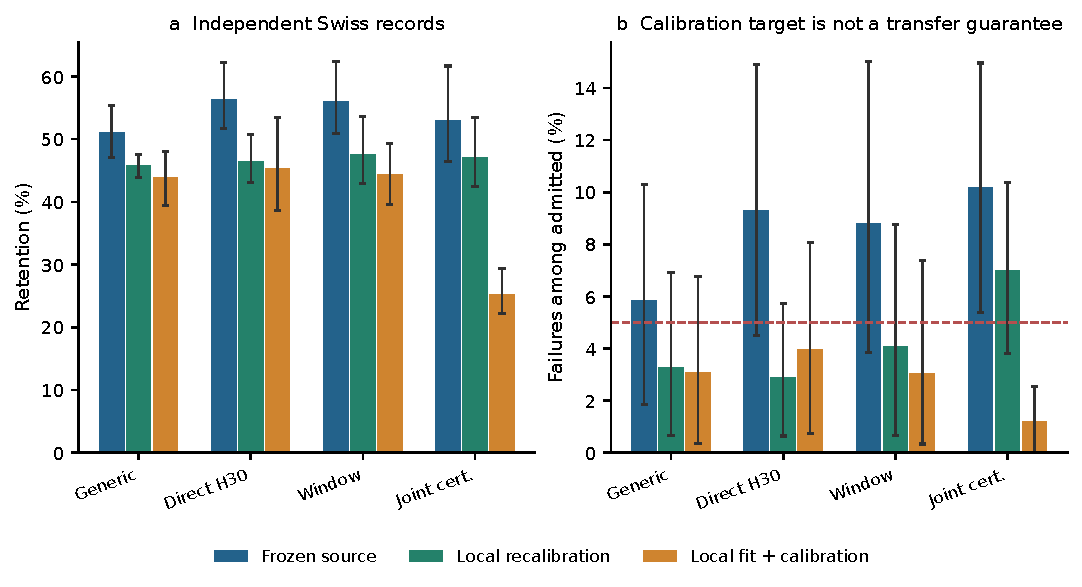
\includegraphics[width=\textwidth]{figures/r3_f4_transfer.pdf}
\caption{Independent Swiss transfer. Source model and threshold are frozen in F0; only target calibration changes in F1; F2 fits on new development stations and calibrates locally. The joint certificate chooses its own reconstruction; other arms deliver the common point. Bars show descriptive test-component bootstrap uncertainty, not distribution-free guarantees. The horizontal calibration target is exceeded after unchanged transfer.}
\label{fig:transfer}
\end{figure}

\subsection{Refusal has a use-dependent benefit and an information cost}

For locally hot-year classification, Swiss F0 refuses \RTestRetHotRefusal{}\% of true hot cases, \RTestRetCoolRefusal{}\% of cool cases and \RTestRetOverallRefusal{}\% overall. The earlier opened-panel statement that hot years are not disproportionately refused is not a universal property. Refusal changes both the judged sample and unknown fraction (Figure~\ref{fig:utility}; SI Table S24).

At missed-hot cost five and unknown-answer cost 0.05 relative to a false-hot answer, loss changes by \RTestRetMagnitudeLossDifference{} per original candidate [\RTestRetMagnitudeLossLow{}, \RTestRetMagnitudeLossHigh{}] versus reconstructing all. This is not sufficient to justify the selective policy: its absolute loss is \RTestRetMagnitudeAbsoluteLoss{}, whereas declaring every record unknown costs only 0.05. We added this deterministic comparator in a post-test audit without changing predictions or the predefined cost grid (SI Table S23). Some other declared cells beat both fixed alternatives at their point estimates, not under a simultaneous or measured management-utility guarantee. With inexpensive errors and costly abstention, even the reconstruct-all comparison can reverse. Observed-hot rescue adds only \RTestRetJudgementRescued{} labels here and \RTestPriorJudgementRescued{} prospectively. H3 holds only for its specified reconstruct-all scenario comparison, not a generally superior operational policy.

Recorded-calendar replay limits a benign-outage interpretation too. New eligible calendars are French aggregates, not Swiss documented-mean confirmation. Across \RNaturalCases{} masks in \RNaturalGroups{} components, unscreened failure is \RNaturalObservedRisk{}\%; the source-fitted composition rule predicts \RNaturalPredictedRisk{}\%. These are conditional replay risks, not error prevalence across complete and incomplete monitoring years combined. They neither reproduce the earlier small replay's benign average nor justify a claim that most networks need no screen. Single-network advice and source-only prediction intervals are not certification (SI Table S20).

\begin{figure}
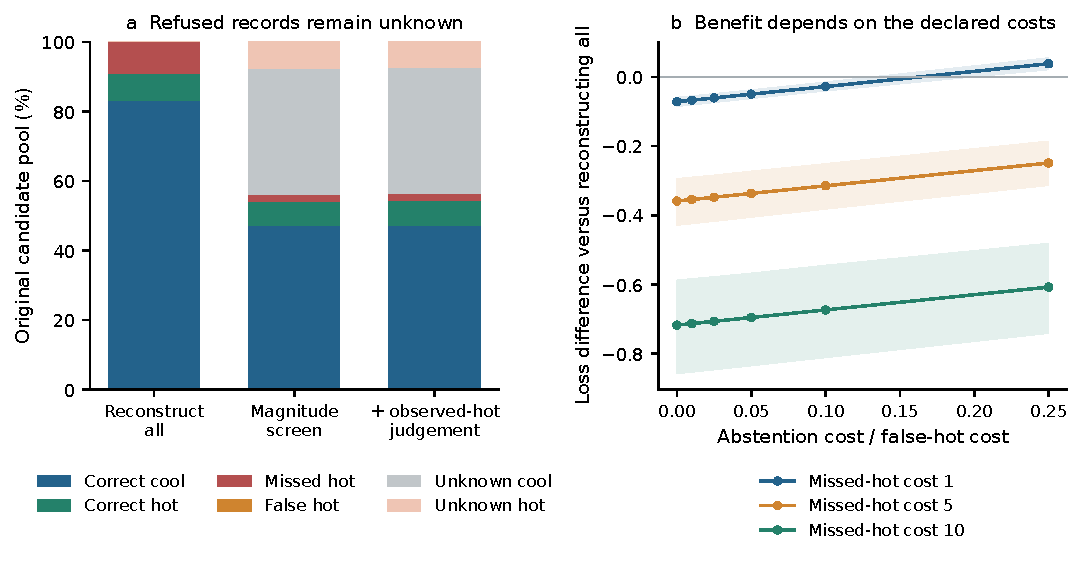
\includegraphics[width=\textwidth]{figures/r3_f5_utility.pdf}
\caption{Original-candidate downstream closure for the frozen Swiss policy and local hot threshold. (a) Correct, mistaken and unknown outcomes retain their denominator. Unknown hot/cool categories use reference truth for evaluation only. (b) Loss differences under declared costs; negative favors screening. Shading is descriptive conditional uncertainty, not simultaneous inference over the grid or a measured valuation of monitoring decisions.}
\label{fig:utility}
\end{figure}


\section{Discussion}

\subsection{What the experiments establish}

The strongest physical result is an interaction between outage position, target statistic and reconstruction information. Missing-day counts are insufficient for H30, but peak overlap is not sufficient either. Explicit support can help transparent rules and restricted models; it is not the necessary component behind the best flexible score. The proposed representation does not establish its intended increment over strong target-specific diagnostics. This negative finding narrows, rather than invalidates, the value of a fit-for-use assessment.

For a fixed point estimate, a complete conditional distribution of H30 would already determine the probability of exceeding its tolerance. Window summaries can help estimate that distribution, but an additional decision signal cannot be assumed. Our direct uncertainty summaries and trajectories are approximations: their observed redundancy is empirical, not a proof that every support representation is useless. Window information may be more relevant to choosing a costly additional data source than to repeatedly summarizing one fixed estimate's risk.

The decomposition makes a separate point: a nonnegative term in a maximum-statistic identity need not describe a harmful process. Switching can compensate a damaged true peak. Centering hidden residuals is likewise diagnostic, not a field method. Interpretation must respect the final sign, intervention interaction and small improvement demonstrated from visible information.

\subsection{Why deployment conditions matter}

New-station tests distinguish ranking from calibration transport. A useful source score can miss its target elsewhere, even with intercontinental river-flow separation. Local calibration changes the problem and may help; it is not successful unchanged transfer. Future station history is legitimate retrospective archive information, not prospective information.

Stream-temperature work already shows that similar in-distribution predictive accuracy need not imply similar performance under environmental shift \cite{topp2023}. Our result concerns transport of an admission calibration, not a demonstration that one neural architecture better represents river processes. Both forms of generalization need tests matching the claimed deployment conditions.

Risk statements must match the independent unit and population. Overlap components prevent duplicate evidence but do not establish independent catchment climates. The formal rule is limited by that assumption and its group-expectation target. No certifiable threshold means insufficient evidence, not that every record is unusable. Nonzero empirical retention cannot be relabelled a guarantee. More masks cannot replace independent calibration groups.

\subsection{Magnitude, judgement and monitoring value}

An agency may need an H30 number, a hot-year label or an unbiased regional frequency. They incur different losses. A refused magnitude can establish hot conditions through a full observed window, but few labels were rescued here. Observations below threshold cannot establish cool conditions. Selected accuracy does not establish representativeness: unknown fractions, hot/cool refusal, coverage and original-pool frequency uncertainty remain outcomes.

The cost grid identifies where screening could help a stated decision. It does not estimate field-revisit costs, ecological losses or the harm of withholding a record. Those require prospective agency-specific work. Our tolerance and finite-history anomaly threshold are experimental choices, not biological standards. We recommend neither a universal archive cutoff nor an assumption that natural outages are harmless.

The main downstream no-screen reference uses the common priority reconstruction. Beating it does not establish a useful selective policy when declaring all answers unknown is cheaper. Any minimum information-return requirement belongs in a prospective utility specification, not a post-test constraint added to defeat that baseline. Scenario benefits also do not establish superiority over an optimally chosen physical reconstruction or information-acquisition policy.

\subsection{Limits and the next independent test}

Opened sources supported development and are not sealed confirmation. Even broader controls require complete training years and do not represent all short, intermittent or persistently gapped records. Missing observations need not be sensor failure: dry channels can change the estimand. Measurement definitions, quality flags and aggregation limit comparability. New histories are European mountain catchments, with few calibration/test components and no within-bundle donor variation. Regulation and groundwater status are unverified.

Calendar replay transfers missing shapes to complete years, not actual hidden observations or an identified MNAR mechanism. Derived and published events differ; incomplete discharge leaves some compound conditions unknown. A corrected snow label creates no new independent examples. Raw trajectory bands miss bias and transfer uncertainty; coverage is measured rather than assumed (SI Table S22).

Power projections stay low for five-point superiority when training/calibration variability is retained, even enlarging only the test set. We stop tuning rather than acquiring stations until a preferred representation wins. A future design should first improve on direct H30 uncertainty and complete historical diagnostics, then freeze predictive and calibration choices and collect independent hydrological and management-use evidence. A favorable subgroup or oracle cannot replace a failed primary comparison.

\section{Conclusions}

Incomplete temperature records should be assessed against an estimand and use, not one completeness percentage. Broad controls establish a substantial position effect while retaining length and reconstruction effects. The identity separates hidden-window error from compensating or harmful switching; oracle intervention does not demonstrate a large usable correction.

The proposed representation does not establish its predefined practical advantage over strong target-specific diagnostics. Unchanged transfer exceeds its nominal target at observed operating points; local recalibration and fitting are different claims. Screening can reduce loss relative to reconstructing all at some declared costs, but always-unknown answers can be cheaper. Unknown records, selected-sample distortion, current-vintage hindcast inputs and small independent cohorts remain part of the result. These distinctions define the present contribution and what a genuinely better design must demonstrate.

\section*{Open Research Statement}

Public products are reused under provider terms. Existing rights and measurement definitions are in \texttt{DATA\_RIGHTS.md}. New contracts, hashes, acquisition records, event/forcing resources and identity exclusions are under \texttt{results/wrr\_submission\_ready/major\_revision\_20261020c/}. The mountain resource has DOI \texttt{10.4211/hs.7a45ee06851e41d99e4affb7110d5f97}; continuous temperatures were reacquired, not inferred from extreme values. Local availability is not permission to redistribute every raw series.

Scripts 348--366 implement protocol, acquisition, recovery, calibration, transfer, references and power; scripts 367--371 and 373 generate final evidence, figures, tables, checks and corrected descriptive strata. Method and deployment locks identify fitted objects and thresholds before test scoring. The protocol and dated nonpredictive erratum are under \texttt{docs/reviews/wrr\_major\_revision\_20261020c/}. Script 368 generates figure sources; script 367 binds numerical macros to result rows and hashes. Previous manuscripts remain superseded history, not current evidence. A permanent archival deposit is required before submission.

\section*{Acknowledgments}
We thank the monitoring agencies and authors of the reused mountain-river resource. Funding, contributions, affiliations and corresponding-author details need verified author input, not inference from repository aliases.


\bibliography{references_r3}
\end{document}
